\subsubsection{XY-Wing}
Die Technik \textit{XY-Wing} wird manchmal auch nur \textit{Y-Wing} genannt, da sie aussieht wie ein \textit{X-Wing} (siehe Kapitel \ref{X-Wing}) nur mit drei Ecken. Zuerst sucht man eine Zelle, in der nur noch 2 Kandidaten verblieben sind. Diese Kandidaten nennt man dann x und y. Daher kommt der im Allgemeinen bekanntere Name der Strategie. Im nächsten Schritt sucht man nun eine Zelle, die in einer gemeinsamen Figur mit der ersten Zelle liegt und auch nur noch 2 Kanididaten der Form hat, dass einer der Kandidaten dem x aus der ersten Zelle entspricht und der zweite Kandidat ungleich dem y ist. Dieser wird nun z genannt. Anschließend sucht man eine dritte Zelle mit nur noch zwei verbliebenen Kandidaten, die ebenfalls in einer gemeinsamen Figur mit der ersten Zelle liegt, aber nicht in der selben wie die zweite gefundene Zelle. Wenn diese Zelle nun die Kandidaten y und z enthält, dann hat man einen \textit{XY-Wing} gefunden. Gelöscht werden kann nun der Kandidat z aus der Zelle, die von der zweiten und dritten Zelle ausgeschlossen wird. Das funktioniert, da in der ersten Zelle entweder x oder y steht. Wenn in der ersten Zelle x steht, dann steht in der zweiten Zelle z, da dort nur x und z stehen kann, x aber durch die erste Zelle ausgeschlossen wird. Wenn in der ersten Zelle aber y steht, dann muss in der dritten Zelle z stehen, da dort nur y und z stehen können und y ausgeschlossen wird. Daher steht in einer der beiden Zellen z und alle Kandidaten von z, die durch beide Felder ausgeschlossen werden, können gelöscht werden.

\begin{figure}[h]
\begin{center}
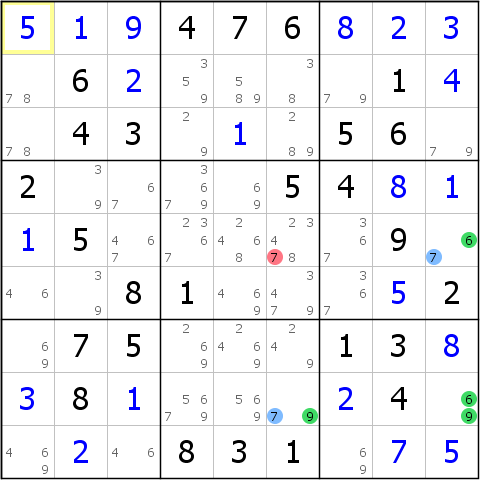
\includegraphics{./img/XY_Wing.png}
\caption{XY-Wing}
\end{center}
\end{figure}

\noindent In \textbf{Abbildung 2.15} stehen in z8s9 die Kandidaten 6 für x und 9 für y. In Zelle z5s9 stehen 6 für x und 7 für z. In z8s6 stehen 9 für y und 7 für z. Wieder werden zwei Fälle getrennt betrachtet. Im ersten Fall nehmen wir an, die Ziffer 7 steht in z5s9. Dann wäre die rot markierte 7 in z5s6 direkt ausgeschlossen, da die beiden Zellen in der selben Zeile liegen. Im zweiten Fall nehmen wir an, die Ziffer 7 steht nicht in z5s9. Dann muss dort die Ziffer 6 stehen. Dadurch muss in z8s9 die Ziffer 9 eingetragen werden, was dazu führt, dass in z8s6 die Ziffer 7 steht und ebenfalls die rot markierte 7 in z5s6 ausschließt. In beiden möglichen Fällen kann die Ziffer 7 also nicht in z5s6 stehen und kann damit gelöscht werden.